\documentclass[pdflatex,sn-mathphys-num]{sn-jnl}

\usepackage{bookmark}
\usepackage{tabularx}
\usepackage{tikz}
\usetikzlibrary{shapes.geometric, shapes.misc, arrows.meta, positioning, calc}
\usepackage{graphicx}
\usepackage{multirow}
\usepackage{amsmath,amssymb,amsfonts}
\usepackage{amsthm}
\usepackage{mathrsfs}
\usepackage[title]{appendix}
\usepackage{xcolor}
\usepackage{textcomp}
\usepackage{manyfoot}
\usepackage{booktabs}
\usepackage{algorithm}
\usepackage{algorithmicx}
\usepackage{algpseudocode}
\usepackage{listings}

\raggedbottom

\begin{document}

\title[Supplementary material: Evaluating CNN vs.\ SVM for Piano Chord Recognition]{Supplementary material: Evaluating CNN vs.\ SVM for Piano Chord Recognition Under Acoustic Domain Shift}

\maketitle

\begin{figure}[htpb]
\centering
\includegraphics[width=\textwidth]{ESM_1.png}
\caption{Web application used to generate and record the dataset via USB MIDI.}
\label{fig:esm-recording-web-app}
\end{figure}

\begin{figure}[htpb]
  \centering
  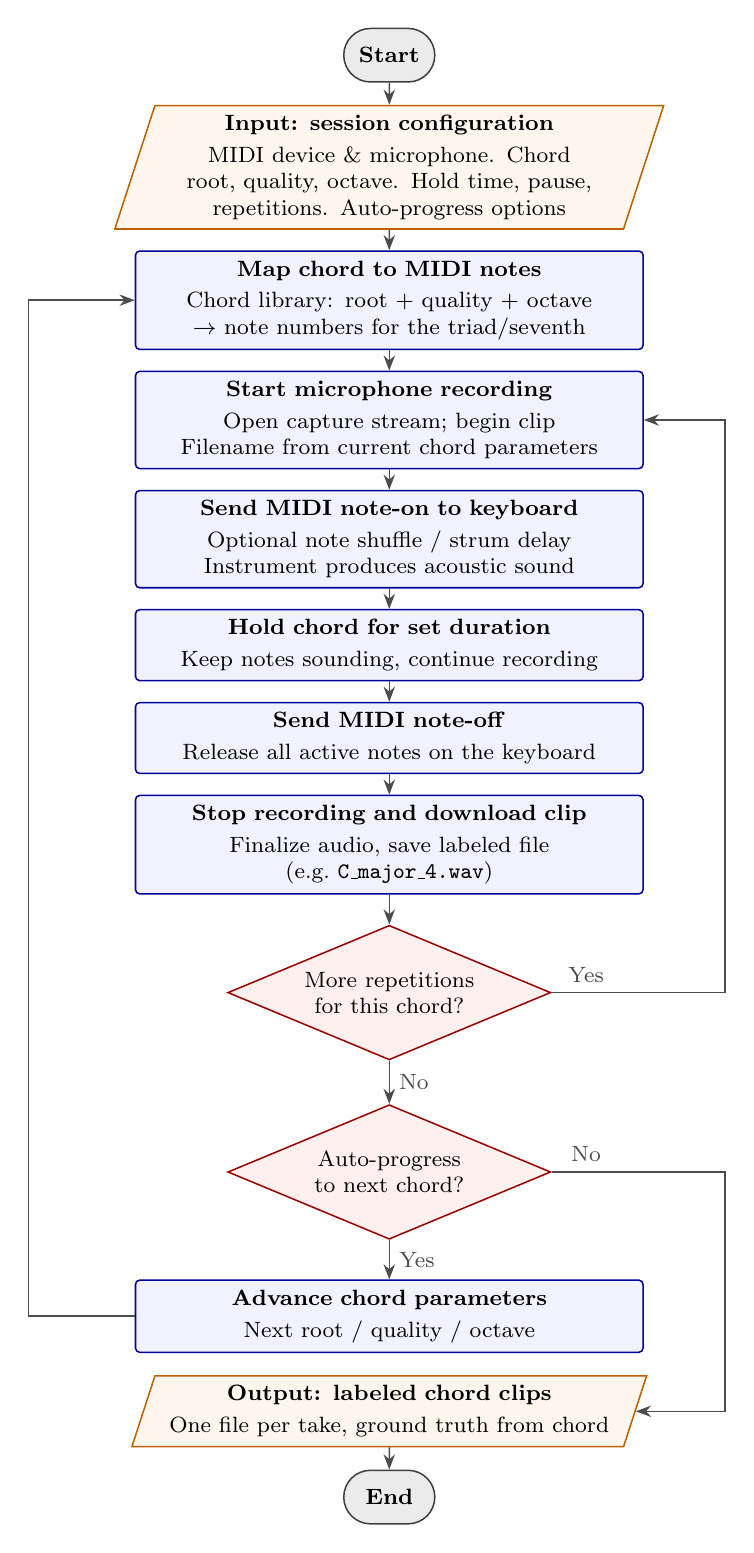
\begin{tikzpicture}[
    node distance=0.22cm and 0.15cm,
    >={Stealth},
    font=\footnotesize,
    base/.style={
      draw, align=center, minimum height=0.55cm,
      line width=0.55pt, inner sep=3.5pt
    },
    terminal/.style={
      base,
      shape=rounded rectangle,
      rounded rectangle arc length=180,
      draw=black!75, fill=black!8,
      minimum height=0.68cm, minimum width=2.0cm,
      inner xsep=12pt, inner ysep=3pt,
      font=\footnotesize\bfseries
    },
    process/.style={
      base, rectangle, rounded corners=1.5pt,
      draw=blue!60!black, fill=blue!5,
      text width=6.2cm
    },
    io/.style={
      base,
      trapezium,
      trapezium left angle=72,
      trapezium right angle=108,
      trapezium stretches body=true,
      draw=orange!75!black, fill=orange!7,
      text width=5.6cm,
      inner xsep=5pt
    },
    decision/.style={
      base,
      diamond,
      aspect=2.4,
      draw=red!60!black, fill=red!6,
      text width=2.6cm,
      inner sep=1pt,
      font=\footnotesize
    },
    arrow/.style={->, line width=0.55pt, black!70}
  ]

    % --- Start ---
    \node[terminal] (start) {Start};

    % --- Configuration ---
    \node[io, below=0.28cm of start] (cfg)
    {\textbf{Input: session configuration}\\[2pt]
     MIDI device \& microphone.
     Chord root, quality, octave.
     Hold time, pause, repetitions.
     Auto-progress options};

    % --- Map chord ---
    \node[process, below=0.26cm of cfg] (map)
    {\textbf{Map chord to MIDI notes}\\[2pt]
     Chord library: root $+$ quality $+$ octave\\
     $\rightarrow$ note numbers for the triad/seventh};

    % --- Start record ---
    \node[process, below=0.26cm of map] (recstart)
    {\textbf{Start microphone recording}\\[2pt]
     Open capture stream; begin clip\\
     Filename from current chord parameters};

    % --- MIDI on ---
    \node[process, below=0.26cm of recstart] (noteon)
    {\textbf{Send MIDI note-on to keyboard}\\[2pt]
     Optional note shuffle / strum delay\\
     Instrument produces acoustic sound};

    % --- Hold ---
    \node[process, below=0.26cm of noteon] (hold)
    {\textbf{Hold chord for set duration}\\[2pt]
     Keep notes sounding, continue recording};

    % --- MIDI off ---
    \node[process, below=0.26cm of hold] (noteoff)
    {\textbf{Send MIDI note-off}\\[2pt]
     Release all active notes on the keyboard};

    % --- Stop + download ---
    \node[process, below=0.26cm of noteoff] (recstop)
    {\textbf{Stop recording and download clip}\\[2pt]
     Finalize audio, save labeled file\\
     (e.g.\ \texttt{C\_major\_4.wav})};

    % --- Decision: more reps? ---
    \node[decision, below=0.38cm of recstop] (morep)
    {More repetitions for this chord?};

    % --- Decision: next chord? ---
    \node[decision, below=0.55cm of morep] (morec)
    {Auto-progress to next chord?};

    % --- Advance chord ---
    \node[process, below=0.5cm of morec] (advance)
    {\textbf{Advance chord parameters}\\[2pt]
     Next root / quality / octave};

    % --- Output summary ---
    \node[io, below=0.28cm of advance] (doneio)
    {\textbf{Output: labeled chord clips}\\[2pt]
     One file per take, ground truth from chord};

    % --- End ---
    \node[terminal, below=0.28cm of doneio] (endn) {End};

    % --- Main vertical path ---
    \draw[arrow] (start) -- (cfg);
    \draw[arrow] (cfg) -- (map);
    \draw[arrow] (map) -- (recstart);
    \draw[arrow] (recstart) -- (noteon);
    \draw[arrow] (noteon) -- (hold);
    \draw[arrow] (hold) -- (noteoff);
    \draw[arrow] (noteoff) -- (recstop);
    \draw[arrow] (recstop) -- (morep);

    % Yes: more reps → back to record (same chord)
    \draw[arrow] (morep.east) -- ++(2.2,0) node[above, font=\footnotesize, pos=0.2] {Yes}
      |- (recstart.east);

    % No: check next chord
    \draw[arrow] (morep) -- (morec) node[midway, right, font=\footnotesize] {No};

    % Yes: next chord → advance → remap
    \draw[arrow] (morec) -- (advance) node[midway, right, font=\footnotesize] {Yes};
    \draw[arrow] (advance.west) -- ++(-1.35,0)
      |- (map.west);

    % No: finished
    \draw[arrow] (morec.east) -- ++(2.2,0) node[above, font=\footnotesize, pos=0.2] {No}
      |- (doneio.east);
    \draw[arrow] (doneio) -- (endn);

  \end{tikzpicture}
  \caption{Detailed application flowchart for the main piano-chord dataset generator.
  The user configures a session; each chord is mapped to MIDI notes, recorded while the
  keyboard is driven over MIDI, then saved as a labeled clip. The loop continues over
  repetitions and auto-progressed chord parameters until the selected set is complete.}
  \label{fig:application-flow-detailed}
\end{figure}

\begin{figure}[h]
\centering
\includegraphics[width=\textwidth]{ESM_2.eps}
\caption{Audio duration distribution across classes in the training dataset.
\textbf{(A)}~major;
\textbf{(B)}~minor;
\textbf{(C)}~diminished.
Variation arises from randomized note attack delays of 0--150\,ms.}
\label{fig:esm-audio-duration-dist}
\end{figure}

\begin{figure}[htpb]
\centering
\includegraphics[width=\textwidth]{ESM_3.eps}
\caption{CNN training and validation curves.
\textbf{(A)}~accuracy;
\textbf{(B)}~loss.
Rapid convergence by epoch 2--3 is consistent with high in-domain CQT discriminability.}
\label{fig:esm-cnn-training-curves}
\end{figure}

\begin{figure}[htpb]
\centering
\includegraphics[width=0.75\textwidth]{ESM_4.eps}
\caption{CNN in-domain test confusion matrix (720 samples, 20 per class).
Perfect diagonal dominance confirms zero misclassifications across all 36 classes.}
\label{fig:esm-cnn-test-confusion}
\end{figure}

\begin{table*}[h]
\caption{CNN in-domain 5-fold cross-validation results with loss}
\label{tab:esm-cnn-kfold-full}
\begin{tabular*}{\textwidth}{@{\extracolsep\fill}llllllll}
\toprule
 & & \multicolumn{3}{l}{Accuracy} & \multicolumn{3}{l}{Loss} \\
\cmidrule(lr){3-5} \cmidrule(lr){6-8}
Fold & Epochs & Train & Validation & Test & Train & Validation & Test \\
\midrule
Fold 1 & 11 & 0.9979 & 1.0000 & 1.0000 & 0.0051 & 0.0000 & 0.0003 \\
Fold 2 & 21 & 0.9979 & 1.0000 & 1.0000 & 0.0051 & 0.0000 & 0.0000 \\
Fold 3 & 19 & 0.9969 & 1.0000 & 1.0000 & 0.0063 & 0.0000 & 0.0000 \\
Fold 4 & 15 & 0.9967 & 1.0000 & 1.0000 & 0.0091 & 0.0000 & 0.0000 \\
Fold 5 & 14 & 0.9985 & 1.0000 & 1.0000 & 0.0058 & 0.0000 & 0.0001 \\
Mean   & 16.0 & 0.9976 & 1.0000 & 1.0000 & 0.0074 & 0.0000 & 0.0001 \\
Std.   & 3.58 & 0.0007 & 0.0000 & 0.0000 & 0.0020 & 0.0000 & 0.0001 \\
\bottomrule
\end{tabular*}
\end{table*}

\begin{figure}[h]
\centering
\includegraphics[width=\textwidth]{ESM_5.eps}
\caption{CNN 5-fold cross-validation training curves.
\textbf{(A)}~accuracy per fold (solid: train, dashed: validation);
\textbf{(B)}~loss per fold.}
\label{fig:esm-cnn-kfold-curves}
\end{figure}

\begin{table*}[h]
\caption{SVM Optuna hyperparameter search: per-fold and mean CV accuracy}
\label{tab:esm-svm-optuna-trials-full}
\begin{tabular*}{\textwidth}{@{\extracolsep\fill}lllllllll}
\toprule
Trial & $C$ & $\gamma$ & Fold 1 & Fold 2 & Fold 3 & Fold 4 & Fold 5 & Mean \\
\midrule
0 & 1 & 0.001 & 0.9961 & 0.9969 & 0.9969 & 0.9985 & 0.9977 & 0.9972 \\
1 & 10 & 0.01 & 0.0324 & 0.0316 & 0.0324 & 0.0355 & 0.0324 & 0.0329 \\
2 & 10 & 0.001 & 0.9961 & 0.9969 & 0.9969 & 0.9985 & 0.9977 & 0.9972 \\
3 & 100 & 0.001 & 0.9961 & 0.9969 & 0.9969 & 0.9985 & 0.9977 & 0.9972 \\
4 & 10 & 0.001 & 0.9961 & 0.9969 & 0.9969 & 0.9985 & 0.9977 & 0.9972 \\
5 & 0.1 & 0.00001 & 0.9738 & 0.9722 & 0.9722 & 0.9776 & 0.9745 & 0.9741 \\
6 & 1 & 0.01 & 0.0324 & 0.0316 & 0.0324 & 0.0355 & 0.0324 & 0.0329 \\
7 & 1000 & 0.0001 & 1.0000 & 1.0000 & 1.0000 & 1.0000 & 1.0000 & 1.0000 \\
8 & 1 & 0.01 & 0.0324 & 0.0316 & 0.0324 & 0.0355 & 0.0324 & 0.0329 \\
9 & 0.1 & 0.0001 & 0.9900 & 0.9907 & 0.9931 & 0.9954 & 0.9915 & 0.9921 \\
\bottomrule
\end{tabular*}
\end{table*}

\begin{figure}[h]
\centering
\includegraphics[width=0.75\textwidth]{svm_training_confusion_matrix.eps}
\caption{SVM in-domain test confusion matrix (720 samples, 20 per class).
Perfect diagonal dominance confirms zero misclassifications across all 36 classes.}
\label{fig:esm-svm-test-confusion}
\end{figure}

\begin{table*}[h]
\caption{CNN misclassification analysis on the evaluation dataset.
Root~$\Delta$ is the root note shift in semitones (true $\to$ predicted).}
\label{tab4_4}
{\small
\begin{tabular*}{\textwidth}{@{}lllrrll@{}}
\toprule
True class & Predicted class & Count & Root $\Delta$ & True-only notes & Pred-only notes \\
\midrule
G$\sharp$\_diminished\_4 & C$\sharp$\_diminished\_4 & 36 & $+5$ & D, G$\sharp$, B & C$\sharp$, E, G \\
D\_minor\_4              & B\_diminished\_4         & 33 & $-3$ & A               & B \\
E\_diminished\_4         & D$\sharp$\_major\_4      & 30 & $-1$ & E               & D$\sharp$ \\
A$\sharp$\_diminished\_4 & B\_diminished\_4         & 20 & $+1$ & C$\sharp$, E, A$\sharp$ & D, F, B \\
C\_diminished\_4         & B\_minor\_4              & 16 & $-1$ & C, D$\sharp$    & D, B \\
F$\sharp$\_minor\_4      & G\_minor\_4              &  5 & $+1$ & C$\sharp$, F$\sharp$, A & D, G, A$\sharp$ \\
G$\sharp$\_diminished\_4 & G\_diminished\_4         &  4 & $-1$ & D, G$\sharp$, B & C$\sharp$, G, A$\sharp$ \\
E\_minor\_4              & G\_minor\_4              &  3 & $+3$ & E, B            & D, A$\sharp$ \\
B\_major\_4              & A$\sharp$\_minor\_4      &  2 & $-1$ & D$\sharp$, F$\sharp$, B & C$\sharp$, F, A$\sharp$ \\
B\_major\_4              & G\_minor\_4              &  2 & $-4$ & D$\sharp$, F$\sharp$, B & D, G, A$\sharp$ \\
A$\sharp$\_diminished\_4 & C\_diminished\_4         &  2 & $+2$ & C$\sharp$, E, A$\sharp$ & C, D$\sharp$, F$\sharp$ \\
G$\sharp$\_minor\_4      & D$\sharp$\_diminished\_4 &  1 & $-5$ & G$\sharp$, B    & F$\sharp$, A \\
F\_diminished\_4         & D\_diminished\_4         &  1 & $-3$ & B               & D \\
F\_diminished\_4         & C$\sharp$\_major\_4      &  1 & $-4$ & B               & C$\sharp$ \\
E\_minor\_4              & F$\sharp$\_major\_4      &  1 & $+2$ & E, G, B         & C$\sharp$, F$\sharp$, A$\sharp$ \\
E\_major\_4              & D$\sharp$\_major\_4      &  1 & $-1$ & E, G$\sharp$, B & D$\sharp$, G, A$\sharp$ \\
C\_major\_4              & A\_major\_4              &  1 & $-3$ & C, G            & C$\sharp$, A \\
A\_major\_4              & C$\sharp$\_major\_4      &  1 & $+4$ & E, A            & F, G$\sharp$ \\
A$\sharp$\_major\_4      & G\_diminished\_4         &  1 & $-3$ & D, F            & C$\sharp$, G \\
\bottomrule
\end{tabular*}
}
\end{table*}

\end{document}
